\section{Initial studies}

\begin{frame}{Initial studies: bibliographic research}
  \begin{columns}[onlytextwidth]
    \begin{column}{0.5\textwidth} 
        \begin{enumerate}
            \item Importance of an electrocardiograph (ECG) instrument;
            \item Electrical and physical characteristics of an ECG signal;
            \item Distortions associated with the ECG;
            \item Consolidated data acquisition systems for ECG;
            \item User interface with the ECG instrument;
        \end{enumerate}
      \end{column}
      
      \begin{column}{0.5\textwidth}
          \begin{figure}[H]
          \caption{Normal waveform pattern of cardiac signal obtained in ECG. Source: \cite{khandpur2019compendium}.}          \begin{center}
                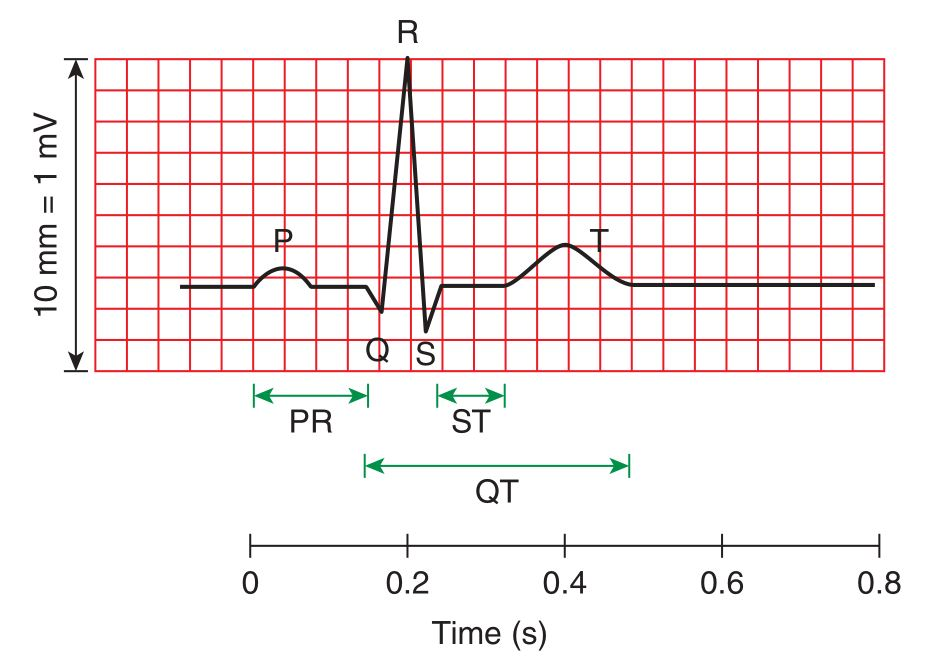
\includegraphics[width=6cm]{images/cardiac_signal.JPG}  
            \end{center}
            \label{fig:1} 
            \end{figure}
      \end{column}
  \end{columns}
\end{frame}

\begin{frame}{Initial studies: system specification}
\begin{minipage}[c][0.5\textheight][c]{\linewidth}
  \begin{columns}[onlytextwidth]
    \begin{column}{\textwidth} 
        \begin{enumerate}
            \item Amplitude:
            \begin{itemize}
                \item ECG signal with $1 \, mV$ peak-to-peak \cite{khandpur2019compendium};
                \item Combined distortions with $\approx 10 \, \mu V$ peak-to-peak \cite{khandpur1987handbook};
                \item \textbf{Solution:} preamplifier gain of 500 \cite{khandpur2019compendium} and $\text{CMRR}>+100dB$ \cite{khandpur2019compendium, khandpur2005biomedical}
            \end{itemize}
            \item Frequency range:
            \begin{itemize}
                \item Typical range $0.05$ to $150 \, Hz$ and sampling rate of $300 \, \text{samples/s}$;
                \item \textbf{Solution:} used sampling rate of $500 \, \text{samples/s}$;
            \end{itemize}
            \item Quantization:
            \begin{itemize}
                \item 16-bit or 24-bit ADC \cite{khandpur2019compendium};
                \item \textbf{Solution:} available 12-bit ADC;
            \end{itemize}
            \item Typical use of bipolar leads arrangement \cite{khandpur2019compendium};
        \end{enumerate}
      \end{column}

  \end{columns}
    \end{minipage}
\end{frame}

\begin{frame}{Initial studies: distortions specifications}
\begin{minipage}[c][0.5\textheight][c]{\linewidth}
  \begin{columns}[onlytextwidth]
    \begin{column}{\textwidth} 
        \begin{enumerate}
            \item Power-line interference:
            \begin{itemize}
                \item Frequency of $50/60 \, Hz$;
                \item \textbf{Solution:} analog Notch filter;
            \end{itemize}
            \item Baseline wanders and muscle contraction:
            \begin{itemize}
                \item Range of $0.05 \, Hz$ \cite{khandpur2019compendium, murugappan2014development} to $0.5 \, Hz$ \cite{sahin2020instrumentation};
                \item \textbf{Solution:} analog high-pass filter;
            \end{itemize}
            \item Electromagnetic interference:
            \begin{itemize}
                \item Higher frequencies (RF);
                \item \textbf{Solution:} analog low-pass filter;
            \end{itemize}
            \item AWGN and aliasing:
            \begin{itemize}
                \item Across all frequency range;
                \item \textbf{Solution:} analog low-pass filter and digital moving average filter;
            \end{itemize}
        \end{enumerate}
      \end{column}

  \end{columns}
  \end{minipage}
\end{frame}







